\renewcommand{\d}{\mathrm d}
\subject{ESPResSo Tutorial}
\title{Visualization of simulation results obtained with \ES{}
} \author{ Georg Rempfer \thanks{\ttfamily 
georg@icp.uni-stuttgart.de}}
\date{\today}
\publishers{Institute for Computational Physics, University of Stuttgart}
\maketitle 
\begin{center}
  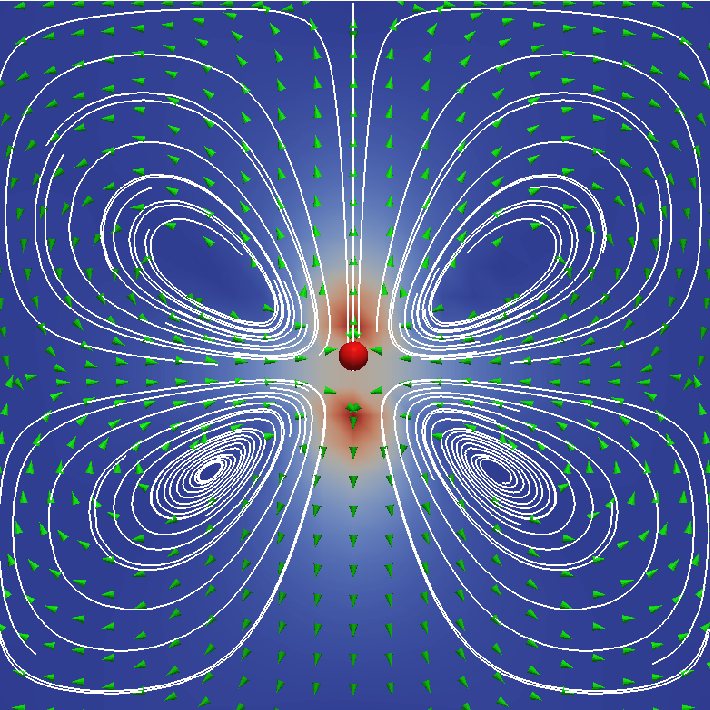
\includegraphics[width=0.5\columnwidth]{figures/flow_field.pdf}
\end{center}
\pagebreak
\definecolor{mygray}{gray}{.75}

 \tableofcontents
 \pagebreak
  
\section{Introduction}

%\floatingBox{5}{4cm}{Mein Text der in der Box abgebildet werden soll. Mal schauen wie das klappt.} 

Whether you are debugging a crashing simulation, trying to understand your simulation results, or create material to explain your findings to fellow researchers -- you are going to require ways to visualize what is going on in your system. Traditionally \ES{} has offered an interface to VMD (Visual Molecular Dynamics), a visualization package developed with NIH support by the Theoretical and Computational Biophysics group at the Beckman Institute, University of Illinois at Urbana-Champaign~\cite{vmd}.

While VMD is an incredibly powerful tool to visualize particle based data, it does not allow the user to include field data such as flow fields produced by coupled MD-LB simulations. To overcome this limitation, the lattice-Boltzmann and electrokinetics implementations in \ES{} contain output routines producing Paraview compatible VTK files. Routines to output particle positions exist as well, which allow the user to produce images and videos of coupled MD-continuum simulations.

\subsection*{Tutorial Outline}

At this stage, the tutorial only contains instructions on how to use Paraview with \ES{} generated data. Please to the User's Guide for information on how to visualize \ES{} simulations with VMD.

\pagebreak
